\documentclass[a4paper, 11pt, twocolumn]{article}

\usepackage[utf8]{inputenc}

\usepackage[T1]{fontenc}

\usepackage[english]{babel}

\usepackage{graphicx}

 \usepackage{floatrow}
 
 \usepackage{caption}
 \usepackage{subcaption}

\usepackage[margin = 1in]{geometry}

\usepackage{float}

\usepackage[hidelinks]{hyperref}


\usepackage{url}

\usepackage[numbers]{natbib}
\usepackage{enumitem}
\bibliographystyle{unsrtnat}
%\usepackage[
%backend=biber,
%sorting=none
%]{biblatex}

%\setcitestyle{authoryear,open={(},close={)}}

\usepackage[most]{tcolorbox}

\usepackage{csquotes}

\usepackage{fancyhdr}


\usepackage{lipsum}

\usepackage{multicol}
%\addbibresource{references.bib}
\title{\Large Methods in Bioinformatics [INFO-F439] Project \\
\huge Review of "muscat detects subpopulation-specific state transitions from multi-sample multi-condition single-cell transcriptomics data"}


\author{Léopold Guyot}

\date{\today}

\begin{document}

\pagestyle{fancy}
\setlength{\headheight}{25.0117pt}
\fancyhead{}\fancyfoot{}
\fancyhead[L]{
\includegraphics[width = 0.2\textwidth]{img/LOGO_Universite__libre_bruxelles.png}}
\fancyhead[R]{Methods in Bioinformatics (INFO-F439) Project}
\fancyfoot[R]{\thepage}


\fancypagestyle{plainfooter}{
	\fancyhf{}  % Clear all headers and footers
	\fancyfoot[R]{\thepage}  % Page number in right footer
}

\onecolumn
\vspace*{-1.5cm}  % Adjust this value as needed
\begin{center}
	{\Large Methods in Bioinformatics (INFO-F439)  Project}\\[1ex]
	{\huge Review of "muscat detects subpopulation-specific state transitions from multi-sample multi-condition single-cell transcriptomics data" \cite{crowell2020muscat}}\\[2ex]
	{\large Léopold Guyot}\\[1ex]
	{\today}
\end{center}
 
\thispagestyle{plainfooter}
%\begin{tcolorbox}[breakable,colback=white,colframe=black,width=\dimexpr\textwidth+12mm\relax,enlarge left by=-6mm]

%\section*{Abstract}


%\end{tcolorbox}


\begin{multicols}{2}
\section{Introduction}

Single-cell RNA sequencing (scRNA-seq) has revolutionised transcriptomics by enabling gene expression profiling at the resolution of individual cells. Unlike bulk RNA-seq, which averages expression signals across thousands or millions of cells, scRNA-seq reveals cell-to-cell heterogeneity and uncovers distinct cellular subpopulations within complex tissues. This allows to provide crucial insights in biological mechanisms.

In many biological and clinical contexts, it is essential to account for this cellular diversity. For instance, in immunology or oncology, the presence or absence of specific cell subtypes can have significant functional and diagnostic implications. A clear example is acute myeloid leukemia (AML), where the tumor comprises a hierarchy of subpopulations, including leukemia stem cells (LSCs) that are often resistant to treatment and responsible for relapse \citep{van2019single}. Identifying and characterising these rare subpopulations is critical for prognosis and therapeutic targeting. scRNA-seq offers the granularity needed to capture such variation, making it indispensable for studies where subtle but biologically meaningful differences may be masked by population averages.

However, the analytical challenges of scRNA-seq data are considerable. The data are high-dimensional, sparse, and noisy due to dropout events and technical variability. Modelling gene expression at the single-cell level must account for these factors while also respecting the hierarchical structure of the data—cells nested within patients or experimental groups. Furthermore, the design of appropriate statistical models must balance sensitivity, specificity, and computational scalability.

To address these challenges, a variety of statistical models have been developed. The \texttt{scDD} method \citep{scdd} models gene expression as a mixture of distributions, enabling the detection of differential expression patterns beyond mean shifts, such as changes in modality or proportion. Mixed-effect models  incorporate both fixed effects (e.g., cell subpopulation) and random effects (e.g., patient) to account for intra-patient correlations and nested data structures.

The reviewed article \citep{crowell2020muscat} proposes a pseudobulking approach, where cells are aggregated by the combination of cell subpopulation and patient. This results in a data structure resembling bulk RNA-seq, reducing noise. Once aggregated, well-established bulk RNA-seq methods such as \texttt{limma} \citep{limma}, \texttt{DESeq2} \citep{deseq2}, and \texttt{edgeR} \citep{edger} can be applied for differential expression analysis. This strategy leverages the robustness of bulk models while preserving important biological structure related to both cell type and biological replicates.


In this study, we aim to reproduce and evaluate the results presented in the reviewed paper, which investigated differential expression analysis strategies for scRNA-seq data. In that work, the authors used two real scRNA-seq datasets as the basis for simulating artificial datasets with known, controlled variations. These simulated datasets allowed for rigorous benchmarking of modelling approaches.

The original study compared different strategies: Single-cell methods including \texttt{scDD}, and mixed-effect models and aggregation-based methods, where cells were grouped by patient and subpopulation to produce pseudobulk profiles, then analysed using established bulk RNA-seq tools such as \texttt{limma}, \texttt{DESeq2}, and \texttt{edgeR}. 

In this review, we reproduce the benchmark of the differential expression methods using simulated and real scRNA-seq datasets, compare our findings with existing studies, and explore the literature about pseudobulking.

\section{Methods}

This project was developed using the R programming language \citep{base} and leveraged packages from the Bioconductor repository \citep{bioc}.

\subsection{Datasets}

To evaluate the performance of pseudobulking methods, the datasets used had to meet specific criteria. In particular, each dataset needed to include multiple patients and several identifiable cell subpopulations. These datasets were then used to simulate new data that mimic the original distribution patterns.

\subsubsection{Kang et al. 2018}

The dataset from Kang et al. \citep{kang_multiplexed_2018} consists of single-cell RNA-sequencing profiles of peripheral blood mononuclear cells (PBMCs) collected from 8 human donors. It includes both unstimulated and interferon-$\beta$–stimulated cells.

The original droplet-based scRNA-seq data is publicly available via the Gene Expression Omnibus (GEO) under the accession \url{https://www.ncbi.nlm.nih.gov/geo/query/acc.cgi?acc=GSE96583}. It is also distributed in the \texttt{SingleCellExperiment} format \citep{sce} through the \texttt{ExperimentHub} package \citep{ExperimentHub}, using the accession code: \texttt{EH2259}.

\subsubsection{Mouse LPS}

The second dataset investigates transcriptomic changes in brain tissue from mice subjected to peripheral lipopolysaccharide (LPS) treatment. It includes samples from 4 vehicle-treated and 4 LPS-treated mice.

This dataset was originally published alongside the reviewed paper \citep{crowell2020muscat}. It is accessible via ArrayExpress (accession: E-MTAB-8192) and can also be obtained from the \texttt{ExperimentHub} package \citep{ExperimentHub} with the accession code: \texttt{EH3297}.

\subsubsection{Guo et al. 2018}

Guo et al. \citep{guo_adult_2018} performed single-cell RNA sequencing on approximately 6,500 testicular cells from 3 healthy adult males, using the 10x Genomics Chromium platform.

This dataset was not included in the original benchmarking paper. It was added here as an independent dataset to assess the generalisability and robustness of the results obtained with other datasets. The aim is to evaluate whether similar conclusions can be drawn using a dataset with different biological context and origin.

The dataset is available through the \texttt{CTdata} R package \citep{CTdata}, and can be accessed using the \texttt{testis\_sce} function.


\subsection{Simulation Framework}

To systematically evaluate differential expression analysis methods, we developed a data-driven simulation framework based on a multi-sample, multi-subpopulation scRNA-seq reference dataset. This framework allows for modulation of key parameters, including the number of cells per subpopulation and sample, as well as the type and magnitude of differential expression patterns. Simulations are based on the negative binomial distribution, which is widely used to model scRNA-seq data. Subpopulation- and sample-specific parameters (means, dispersions, and library sizes) are estimated directly from the reference dataset. Simulated data is then generated by sampling from these empirical distributions, thereby capturing the structure and variability observed in real scRNA-seq data.

To introduce biologically meaningful variation, genes can be designated as subpopulation specific (differential across cell types), condition specific (differential expression between treatment conditions), or non-differential (uniform expression across all variables). 

The framework supports a diverse set of expression patterns based on the classification by Korthauer et al. \citep{korthauer2016statistical}:
\begin{itemize}[itemsep=1pt, topsep=1pt]
	\item \textbf{DE (Differential Expression)}: A change in the mean expression level of a gene between conditions, while the overall distribution shape remains unimodal and similar.
	\item \textbf{DP (Differential Proportion)}: A shift in the proportions of cells in low and high expression states between conditions, without a change in the expression values themselves.
	\item \textbf{DM (Differential Modality)}: A change in the modality of gene expression, such as shifting from an unimodal to a bimodal distribution, indicating that the underlying structure of expression changes.
	\item \textbf{DB (Differential Both)}: A combination of DP and DM, where both the proportions and the modality of expression states differ between conditions.
	\item \textbf{EE (Equally Expressed)}: No differences in expression or distribution between conditions or subpopulations; expression is consistent across all samples.
	\item \textbf{EP (Equal Proportion)}: Genes exhibit bimodal expression, but the proportions of cells in each expression state remain the same across conditions.
\end{itemize}

This classification enables simulation of complex and realistic gene expression scenarios, making the framework well-suited for benchmarking modelling methods across a variety of biologically plausible settings.

\subsection{Pseudobulk Approach}

To reduce the complexity of the data to be modeled, an aggregation approach can be applied. This involves summarising the counts of cells belonging to a specific patient and a specific cell group (Fig. \ref{fig:pseudobulk}). Aggregation can be performed using different summary statistics, such as the sum or the mean. By applying this technique, we simplify the data and reduce the noise while preserving meaningful biological variation, specifically the variability between biological replicates and the variability between cell (sub)populations.
\begin{figure}[H]
	\centering
	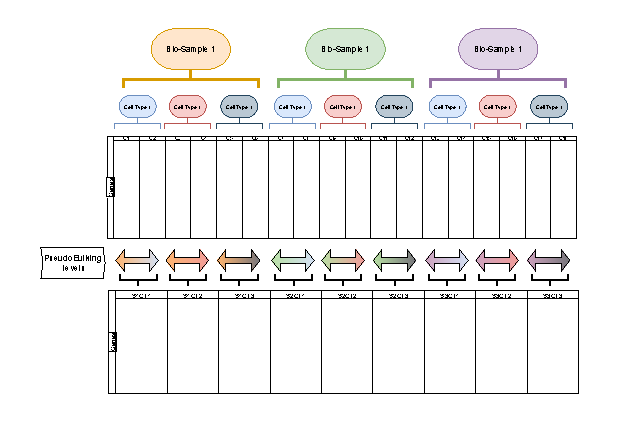
\includegraphics[width=1\columnwidth]{img/rnapseudobulk.drawio-1.pdf}
	\caption{{\footnotesize Scheme of the pseudobulk approach. The columns in the first table represent the individual cells. Several cells belonging to the same bio-sample and cell type are aggregated to give the second table in which each column represent the value for a particular bio-sample and cell type.}}
	\label{fig:pseudobulk}
\end{figure}

\subsection{Workflow}

\begin{figure}[H]
	\centering
	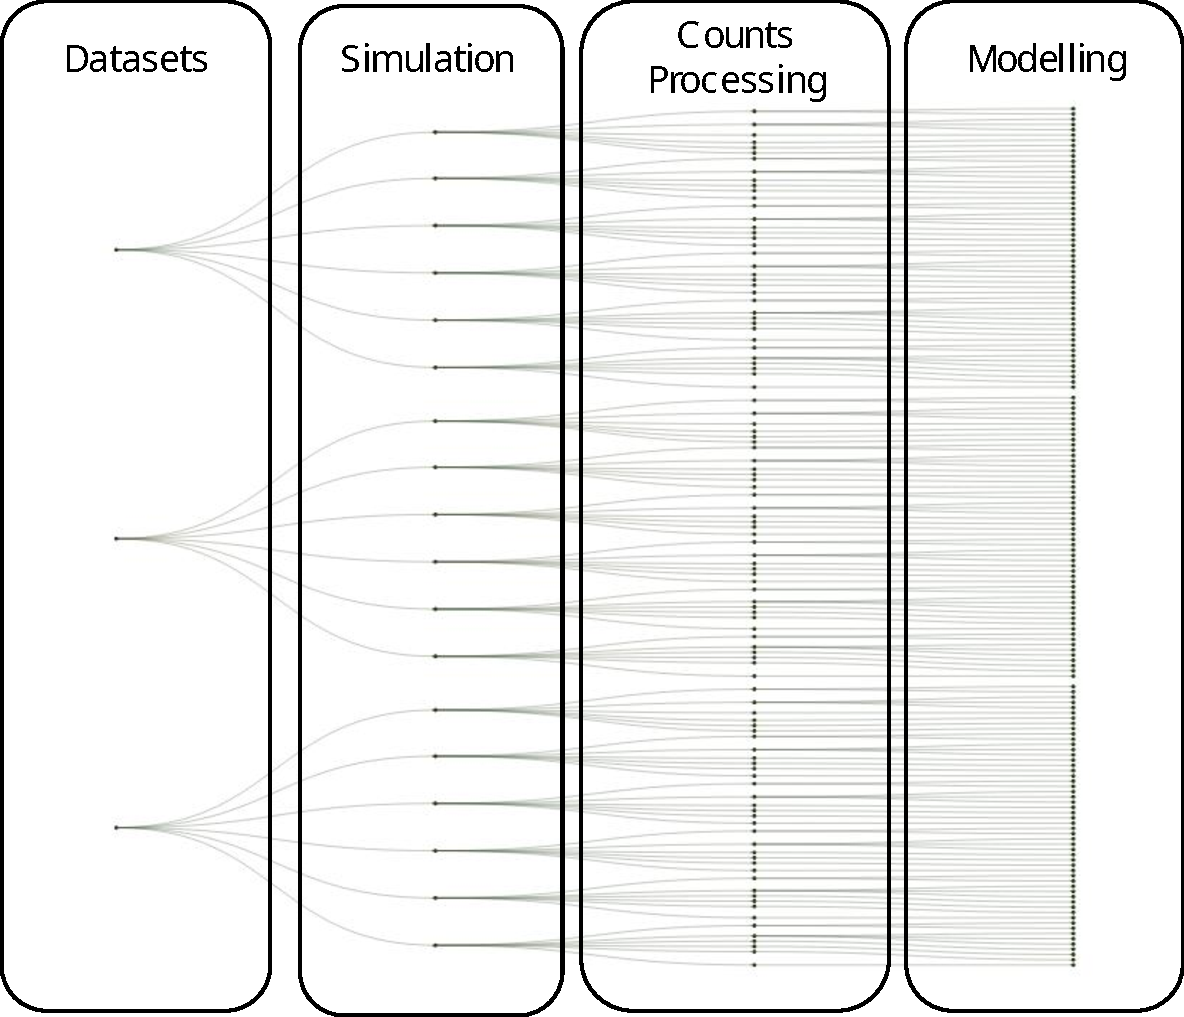
\includegraphics[width=0.7\columnwidth]{img/workflowCut.pdf}
	\caption{{\footnotesize Scheme of the workflow generated with \texttt{targets}. The first layer is the datasets retrieval and preprocessing. The second layer is the simulation of new datasets using different parameters. The third layer is the use of different processing method and aggregation techniques on counts. The fourth layer is the modelisation of the data.}}
	\label{fig:workflow}
\end{figure}

Given the complexity and number of steps involved in this workflow, we used the \texttt{targets} R package \citep{targets} to automate the entire process. Each step is applied to the results produced by all preceding steps, ensuring a consistent and reproducible pipeline. In total, the workflow comprises 291 steps and results in the generation of 144 models (Fig. \ref{fig:workflow}).

\subsubsection{Preprocessing}

Each dataset underwent a standardised preprocessing procedure. To ensure that only the intended variation was present, we retained a single experimental condition per dataset. Specifically, for the Kang et al. dataset, only the control cells were kept; for the mouse LPS dataset, only vehicle-treated cells were retained; and the testis dataset included only one experimental condition.

We filtered genes to retain those with more than one count in at least 10 cells. Similarly, we filtered cells to keep only those expressing at least 100 genes. Additionally, we retained only those clusters that consisted of at least 100 cells.

\subsubsection{Simulation}

The datasets were used to generate artificial data according to the simulation framework described earlier. We used functions provided by the \texttt{muscat} R package \citep{muscat} to facilitate the simulation process.

We simulated various scenarios using different parameter combinations. In the first set of simulations, each sample-subpopulation combination contained 400 cells. We considered four cases:
\begin{enumerate}[itemsep=0pt, topsep=0pt]
	\item 10\% of genes were altered in both proportion and modality (DB).
	\item 10\% of genes were altered in mean expression (DE).
	\item 10\% of genes were altered in modality (DM).
	\item 10\% of genes were altered in the proportions of low and high expression-state components (DP).
\end{enumerate}

Additionally, we conducted a series of simulations in which 10\% of the genes were altered in mean expression, varying the number of cells per sample-subpopulation combination (20, 100, and 400 cells).

\subsubsection{Processing Counts}

Each simulated dataset was processed using multiple count normalisation methods. These included log-transformation, residuals, counts-per-million (CPM), and unprocessed raw counts. The transformations were performed using the \texttt{calculateCPM}, \texttt{normalizeCounts}, and \texttt{computeLibraryFactors} functions from the \texttt{scuttle} R package \citep{scatter}, as well as the \texttt{vst} function from the \texttt{sctransform} R package \citep{sctrans}.

\subsubsection{Pseudobulk}

We applied three different pseudobulk aggregation strategies: mean aggregation, sum aggregation, and no aggregation.

\subsubsection{Modelisation}

We employed a variety of models for differential analysis, using the formula \texttt{\textasciitilde{} patient + cell\_subpopulation}. For non-aggregated data, we applied mixed models and the \texttt{scDD} method. The mixed models were implemented using the \texttt{lmer} function from the \texttt{lme4} package \citep{lme4}, treating the patient effect as a random effect. The \texttt{scDD} method was implemented using the \texttt{scDD} package \citep{scdd}.

For aggregated (pseudobulk) data, we used established bulk RNA-seq modelling approaches, including \texttt{limma} \citep{limma}, \texttt{DESeq2} \citep{deseq2}, and \texttt{edgeR} \citep{edger}. The \texttt{limma} package was applied with either the \texttt{voom} or the \texttt{trend} method.

\subsubsection{Process Results}

The results were processed using the \texttt{iCOBRA} package \citep{icobra}. Differential expression tables were used to generate FDR–TPR curves at various adjusted \textit{p}-value thresholds (0.01, 0.05, 0.1, and 0.2) comparing the results between locally adjusted \textit{p}-value (at the cluster level) and globally adjusted \textit{p}-value. Additionally, UpSet plots were generated to visualise the intersections of detected gene sets across methods and ground truth. The runtime for each method, comprising both the aggregation and modelling steps, was recorded using the \texttt{targets} package \citep{targets}.

\subsection{LPS Downstream Analysis}

In the reviewed article, the researchers also applied downstream analysis to pseudobulked LPS dataset. To reproduce the results we applied the same pseudobulk methods as described before with mean and sum aggegation on the LPS mouse data. Then MDS and UMAP plots were drawn.
\section{Results}

\subsection{Effect of the Variation Type Introduced on Model Performance}

\subsubsection{Kang and LPS datasets}
To assess the impact of different expression variation types on method performance, we here show the simulation results based on the Kang dataset (Fig. \ref{fig:fdrtpr_prop_kang}). Note that the results obtained from the mouse LPS show equivalent results. These simulations introduced distinct categories of gene expression variation. The results are compared based on the true positive rate (TPR) and false discovery rate (FDR) across tested differential state methods.

\textbf{DB (Differential Both)} simulations showed consistently poor TPR across all tested methods. This was expected, as DB genes combine changes in both proportions and modality, presenting a particularly challenging scenario for current models. The inability to detect DB genes highlights the limitations of existing methods in capturing simultaneous changes in expression state prevalence and distribution structure. Even the scDD method which works by comparing the distribution of expression did not successfully model these simulated data.

In contrast, \textbf{DE (Differential Expression)} simulations demonstrated that pseudobulk methods outperformed both mixed models (MM) and scDD. Among the pseudobulk approaches, performance was generally strong, although \textit{limma-trend} applied to VST residuals showed a reduced TPR compared to other pseudobulk variants. scDD exhibited very low TPR. Also locally adjusted p-values improved detection rates, this came at the cost of a notable increase in FDR.

\textbf{DM (Differential Modality)} simulation results were similar to those for DE, with aggregation-based methods again showing superior performance relative to MM and scDD. Notably, scDD, while still exhibiting low TPR, showed improved FDR control in this scenario compared to its performance on DE simulations.

\textbf{DP (Differential Proportion)} was the most challenging variation type among DE, DM, and DP. All methods exhibited a small drop in TPR compared to DE and DM. In particular, \textit{limma-trend} using VST residuals failed to model the data effectively, with especially low TPR.

Overall, these results highlight the clear advantage of pseudobulk-based approaches across various expression variation types, particularly DE and DM. Mixed models and scDD lagged behind, especially in more complex scenarios.

\subsubsection{Impact of Count Processing Strategies}
Across all datasets and variation types, the choice of count processing strategy had minimal impact on model performance for most pseudobulk methods. However, one notable exception was observed for the \textit{limma-trend} method when applied to VST residuals. This count processing method consistently showed reduced TPR and, in some cases, increased FDR, particularly in the DE and DM scenarios.

\subsubsection{Validation on an Independent Dataset: testis dataset} 
To assess the robustness of our observations, we additionally tested all methods with a newly added \textit{testis} dataset (Fig. \ref{fig:fdrtpr_prop_testis}). Globally, the results obtained on this dataset were consistent with those from the Kang and LPS datasets, reinforcing the validity of our conclusions. For most variation types, the relative performance of the methods remained similar. However, a notable deviation was observed for \textbf{DM (Differential Modality)} simulations: the \textit{limma-trend} method applied to VST residuals displayed an elevated FDR, reaching up to 20\% false positives. This suggests that this approach may be unreliable for detecting modality-driven changes in certain biological contexts. Despite this exception, the overall agreement in trends between datasets increases our confidence in the comparative evaluation and the general applicability of the simulation framework.


\subsection{Effect of sample size on model performance}

We assessed the impact of the number of cells per patient and subpopulation on model performance. The results were consistent across all datasets tested: Kang (Fig. \ref{fig:fdrtpr_size}), LPS (data not shown), and testis (Fig. \ref{fig:fdrtpr_testis}). This is confirming the generalisability of the observed trends.

As expected, model performance declined when the number of cells per patient/subpopulation decreased. This effect was evident in both true positive rate (TPR) and false discovery rate (FDR), with fewer cells leading to reduced sensitivity and less stable error control. This is the case for bothe aggregation and non-aggregation methods.
	
\subsection{Runtime Analysis}

\begin{figure}[H]
	\centering
	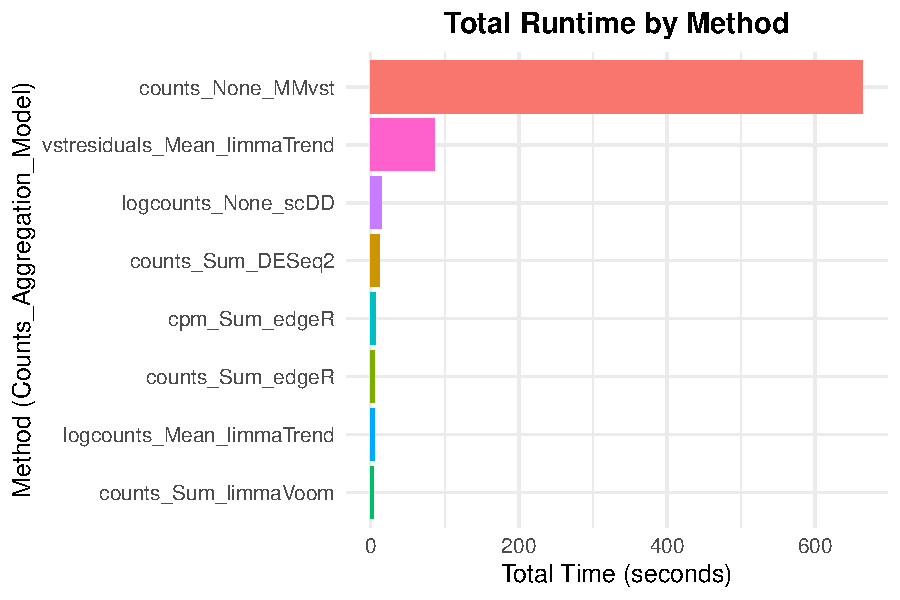
\includegraphics[width=1\columnwidth]{figs/plot_runtime_Kang.pdf}
	\caption{{\footnotesize Runtime analysis for the Kang dataset of the counts processing + aggregation and the modelisation. Time in seconds.}}
	\label{fig:runtime}
\end{figure}

To complement our performance evaluation, we also compared the computational efficiency of the tested methods by measuring their total runtime on the Kang dataset (Fig. \ref{fig:runtime}). The results clearly show that aggregation-based pseudobulk methods are consistently the most efficient. This highlight the scalability and practicality of pseudobulk-based workflows, especially for large single-cell datasets.

While most count processing strategies had little impact on computational time, an exception was observed for the \textit{vstresiduals} used in combination with \textit{limma-trend}, which resulted in increased runtimes and poorer performance compared to other aggregation schemes. 

Notably, methods based on mixed models (\textit{MMvst}) and scDD were the slowest among all those tested, often requiring several times more computational time than pseudobulk approaches. If we take in consideration our earlier findings, these methods did not yield superior performance. Thus they may not justify their higher computational cost in most applications.

Taken together, these results support the recommendation of pseudobulk approaches not only for their accuracy but also for their computational efficiency, making them well-suited for both small and large scale differential state analyses in scRNA-seq studies.

\subsection{LPS Downstream Analysis}

To further validate the reproducibility of the findings from the reviewed study, we performed downstream analysis on the LPS dataset using pseudobulked data. Specifically, we reproduced the MDS and UMAP plots as described in the original article. Here, we focus on the MDS results (Fig. \ref{fig:MDS_plot}).

While the original article presented MDS plots based on sum-aggregated counts, we extended this by generating an MDS plot using mean-aggregated (averaged) expression data. We can make the same observations on both pseudobulk methods. The MDS plots revealed clear clustering by cell type, indicating strong subpopulation identity. However, similar to the observations in the review paper, the separation between treatment conditions (LPS vs. Vehicule) was not pronounced. This suggests that while pseudobulking preserves cell-type-specific expression structure well, it may not always capture subtle treatment effects at the global expression level.

\section{Discussion}

Our benchmark results using the Kang and LPS datasets are in strong agreement with those reported in the reviewed paper. Across both datasets (Kang and LPS), we observed similar trends that reinforce the conclusions from the reviewed article. Notably, pseudobulk approaches consistently outperformed both mixed models (MM) and scDD in terms of true positive rate (TPR) and false discovery rate (FDR). This superior performance was especially clear in the detection of genes with differential expression (DE) and differential modality (DM), where pseudobulk methods yielded both high true positive rates (TPRs) and efficient runtime.

As previously reported, we also observed that scDD exhibited poor performance across most simulated variation types, and that \textit{limma-trend} applied to VST residuals was the least performant among the pseudobulk methods tested. Additionally, our results confirmed the difficulty in detecting DB (differential both) genes, consistent with the original study. These genes, which combine modality and proportion shifts, remain particularly challenging to identify for all evaluated methods. Furthermore, we reproduced the difference between globally and locally adjusted p-values: while local adjustments led to higher sensitivity, they also resulted in inflated FDR.

Importantly, both our analysis and the reviewed article highlighted the critical impact of the number of cells per patient and per subpopulation on model performance. As the number of cells increased, all methods improved in accuracy, but the rate of improvement varied.

To further test the generalisability of our conclusions, we evaluated all methods on an additional dataset derived from testis tissue. Remarkably, the results obtained from this dataset mirrored those from the Kang and LPS datasets, and by extent as those reported in the reviewed article. This consistency across datasets reinforces the robustness of our findings and supports the broader applicability of the conclusions drawn regarding method performance, computational efficiency, and sensitivity to sample size.

Nevertheless, there are important differences between our setup and the one used in the reviewed article that should be acknowledged. For example, we did not replicate each method-simulation pair multiple times as they did, primarily due to computational constraints (our full benchmark already required over eight hours of runtime). Additionally, our benchmark did not cover all models or preprocessing strategies included in their study. In particular, we did not test alternative count processing methods applied to MM or scDD models, nor did we evaluate methods based on Anderson–Darling (AD) tests or MAST, which were used in the original paper.

We also looked at the literature on the pseudobulking subject, we identified an other study by Zimmerman et al. \citep{zimmerman2021practical} that raised concerns regarding the use of pseudobulk methods for single-cell differential analysis. Their simulations, which accounted for intra-individual correlation structures observed in real data, suggested that while pseudobulk approaches provided good type 1 error control, they were overly conservative—leading to inflated type 2 error rates. This was attributed to the loss of information due to aggregation and imbalanced cell numbers across individuals, which disproportionately impacted statistical power. They recommended generalised linear mixed models  with patient random effects as the most effective solution for balancing type 1 and type 2 error control.

However, these findings were critically re-evaluated by Murphy and Skene \citep{murphy2022balanced}, who highlighted important methodological issues in the original analysis. Notably, they pointed out that Zimmerman et al. did not control for randomness in their simulations, making direct comparisons between methods unreliable. Indeed, different methods were not using the same simulated data. Moreover, they emphasised the limitations of evaluating methods solely based on type 1 or type 2 error rates. By introducing other metrics like the Matthews Correlation Coefficient and ROC curves, Murphy and Skene demonstrated that pseudobulk approaches, particularly aggregation by averaging, outperformed all other tested methods, including GLMMs. Even in the presence of imbalanced datasets, mean-based pseudobulking maintained superior performance, challenging the earlier claims of excessive conservatism. These findings reaffirm our conclusions, strengthening the case for pseudobulk methods as a robust and computationally efficient solution for DS analysis in scRNA-seq data.

\section*{Code Availability}

All scripts used for this report are available on \url{https://github.com/leopoldguyot/muscat.Replication}.

\pagebreak
\bibliography{references}
\end{multicols}

\begin{figure}[h]
	\centering
	\begin{subfigure}[t]{0.9\textwidth}
		\centering
		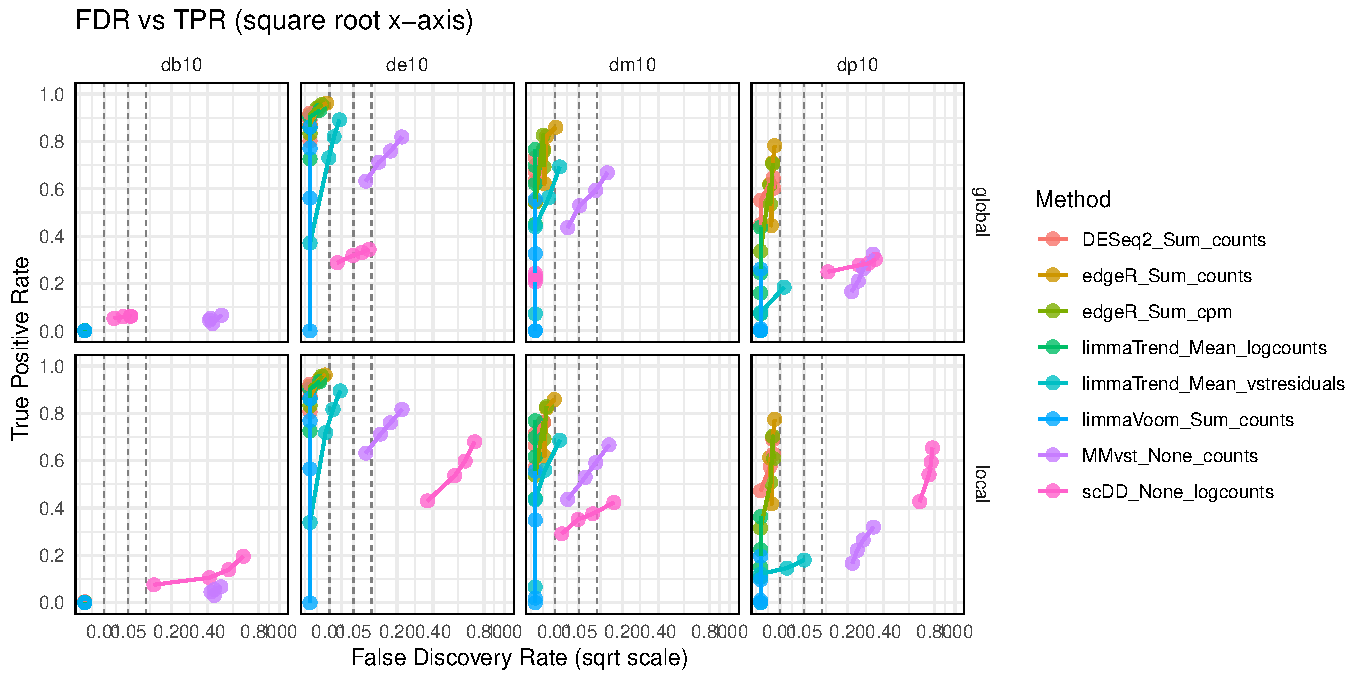
\includegraphics[width=\textwidth]{figs/fdrtpr_prop_method_Kang.pdf}
		\caption{}
		\label{fig:fdrtpr_prop_kang}
	\end{subfigure}
	
	\vspace{1em}
	
	\begin{subfigure}[t]{0.8\textwidth}
		\centering
		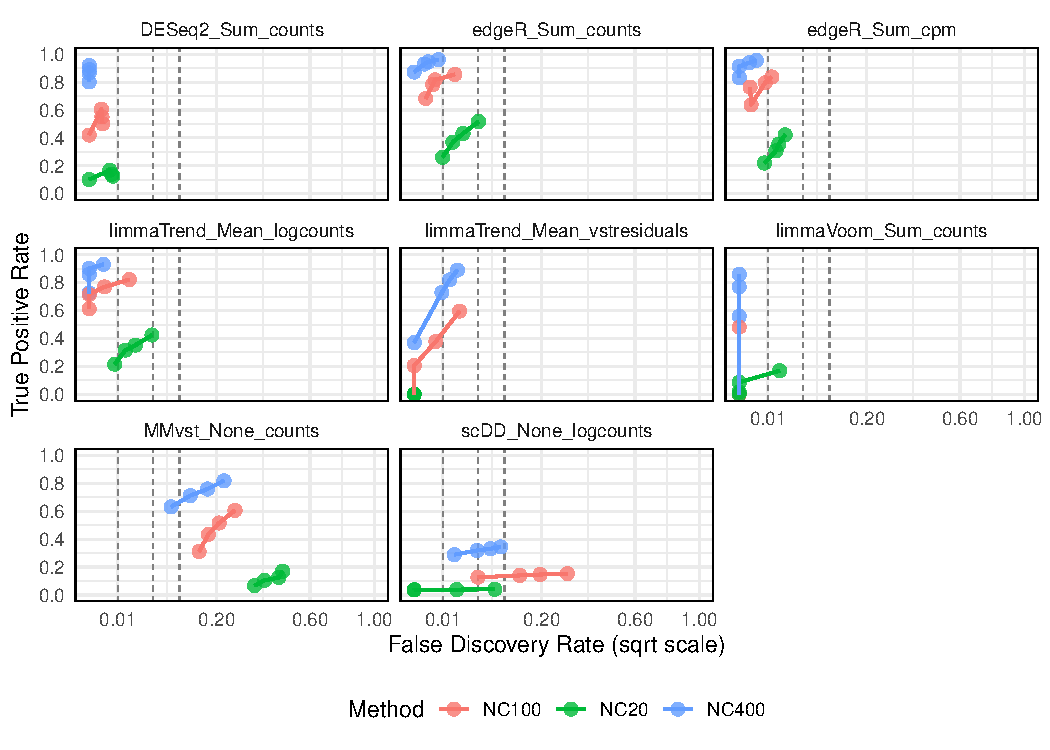
\includegraphics[width=\textwidth]{figs/fdrtpr_size_method_Kang.pdf}
		\caption{}
		\label{fig:fdrtpr_size}
	\end{subfigure}
	
	\caption{{\footnotesize FDR vs TPR of the methods applied on the \textbf{Kang dataset} for different adjusted pvalue thresholds (0.01, 0.05, 0.1 and 0.2). Dashed line represent FDR values of 0.01, 0.05 and 0.1 \textbf{[a]} Comparison for different types of introduced variation. Each column of plots represent a variation type. db10 = 10\% of genes where both the proportions and the modality of expression differ, de10 = 10\% of genes altered in their mean expression between condition, dm = 10\% of genes with a change in the modality of their expression, dp10 = 10\% of genes with a shift in the proportion of cells in low and high expression states between conditions. The first row of plots use globally adjusted pvalues, the second row use locally adjusted pvalues (on each cluster). Colors represent the different methods. \textbf{[b]} Comparison of the performance of the methods with different number of cells by patient and clusters. Performance computed on de10 simulated data and with globally adjusted pvalues. NC20 = 20 cells (green), NC100 = 100 cells (red) and NC400 = 400 cells (blue). Each plot stand for a different method.}}
	\label{fig:fdrtpr_combined_kang}
\end{figure}


\begin{figure}[h]
	\centering
	\begin{subfigure}[t]{0.9\textwidth}
		\centering
		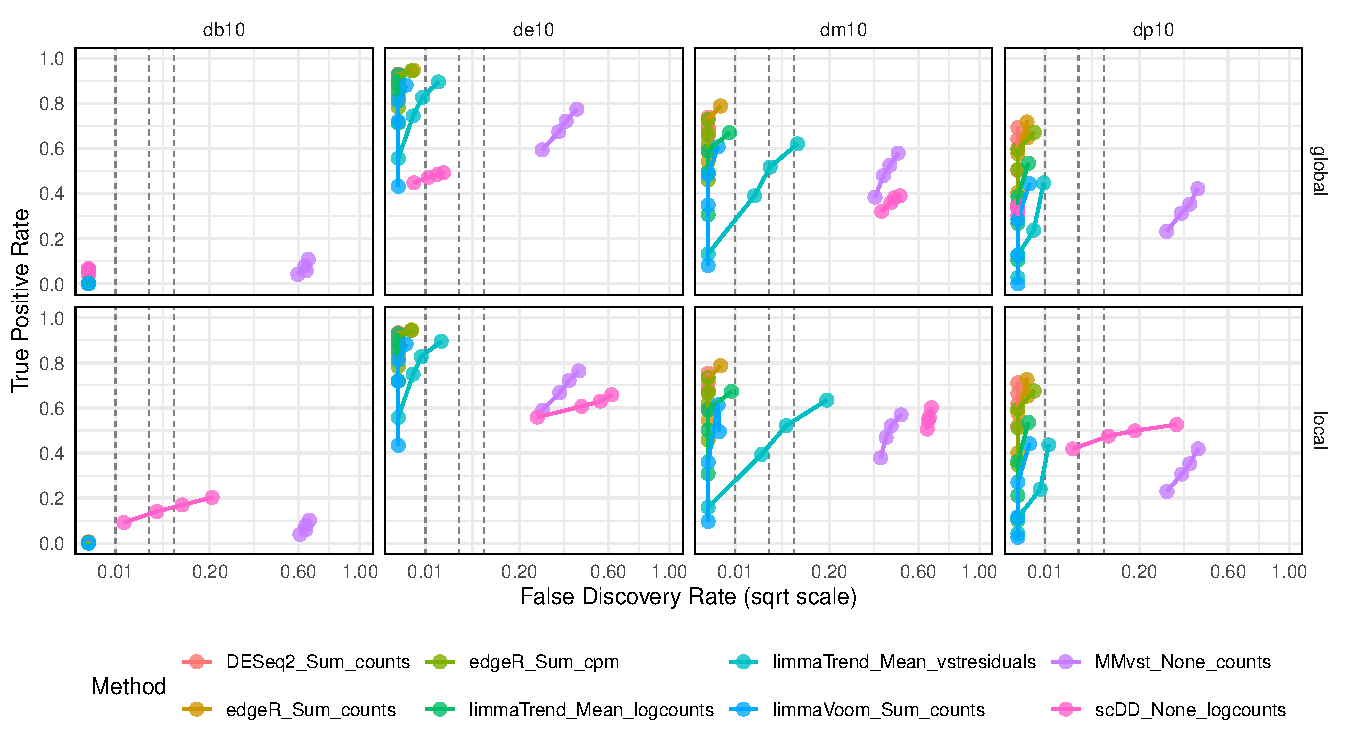
\includegraphics[width=\textwidth]{figs/fdrtpr_prop_method_Testis.pdf}
		\caption{}
		\label{fig:fdrtpr_prop_testis}
	\end{subfigure}
	
	\vspace{1em}
	
	\begin{subfigure}[t]{0.8\textwidth}
		\centering
		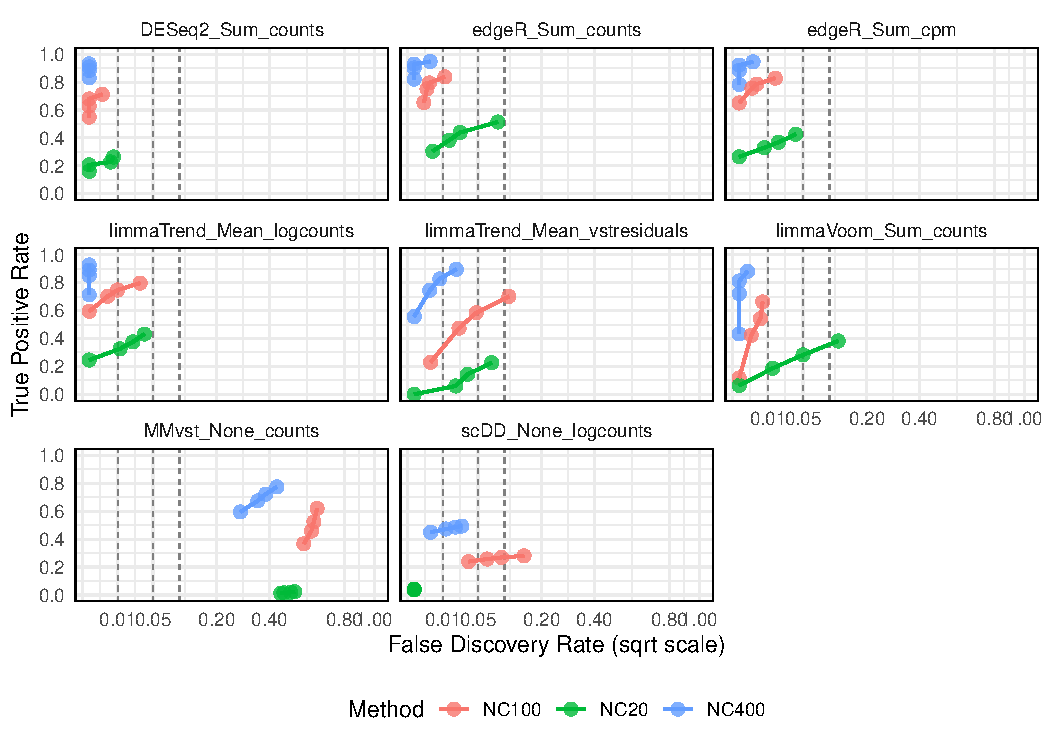
\includegraphics[width=\textwidth]{figs/fdrtpr_size_method_Testis.pdf}
		\caption{}
		\label{fig:fdrtpr_testis}
	\end{subfigure}
	
	\caption{{\footnotesize FDR vs TPR of the methods applied on the \textbf{LPS mouse dataset} for different adjusted pvalue thresholds (0.01, 0.05, 0.1 and 0.2). Dashed line represent FDR values of 0.01, 0.05 and 0.1 \textbf{[a]} Comparison for different types of introduced variation. Each column of plots represent a variation type. db10 = 10\% of genes where both the proportions and the modality of expression differ, de10 = 10\% of genes altered in their mean expression between condition, dm = 10\% of genes with a change in the modality of their expression, dp10 = 10\% of genes with a shift in the proportion of cells in low and high expression states between conditions. The first row of plots use globally adjusted pvalues, the second row use locally adjusted pvalues (on each cluster). Colors represent the different methods. \textbf{[b]} Comparison of the performance of the methods with different number of cells by patient and clusters. Performance computed on de10 simulated data and with globally adjusted pvalues. NC20 = 20 cells (green), NC100 = 100 cells (red) and NC400 = 400 cells (blue). Each plot stand for a different method.}}
	\label{fig:fdrtpr_combined_testis}
\end{figure}

\begin{figure*}[ht]
	\centering
	\begin{subfigure}[t]{0.45\textwidth}
		\centering
		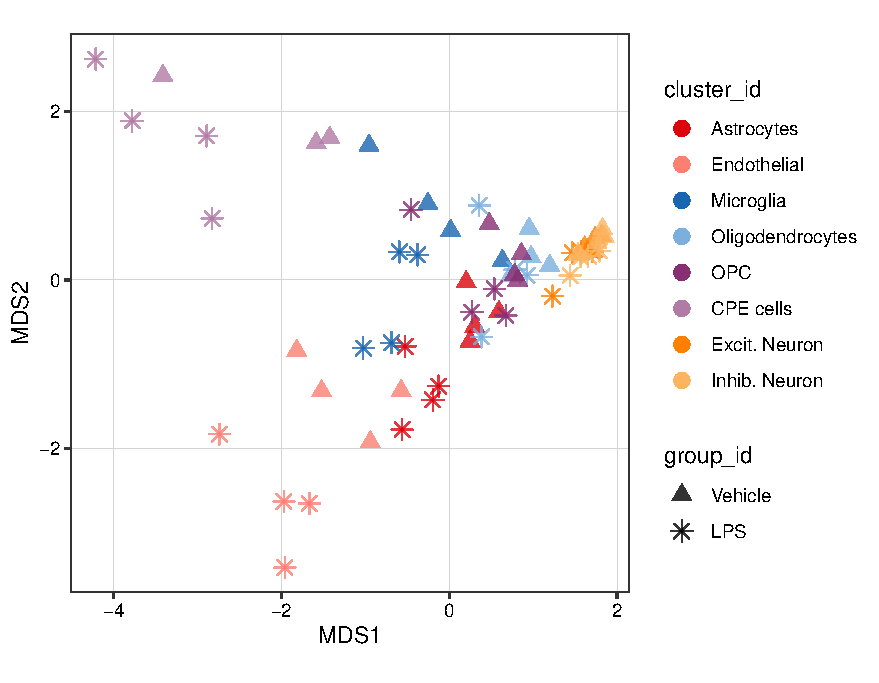
\includegraphics[width=\textwidth]{figs/MDS_LPS_Sum.pdf}
		\caption{Sum Aggregation}
		\label{fig:MDS_Sum}
	\end{subfigure}
	\hfill
	\begin{subfigure}[t]{0.45\textwidth}
		\centering
		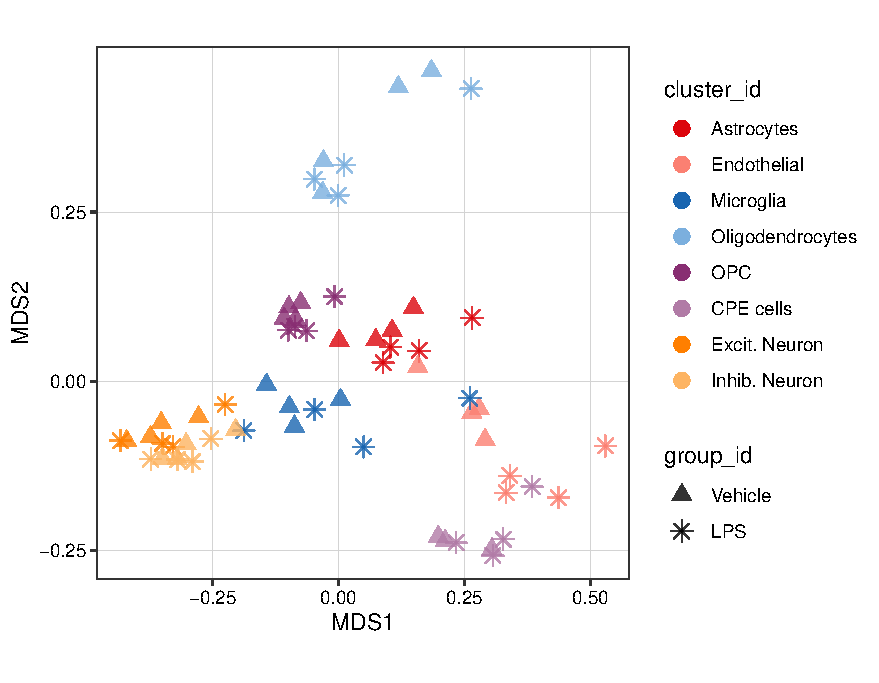
\includegraphics[width=\textwidth]{figs/MDS_LPS_Mean.pdf}
		\caption{Mean Aggregation}
		\label{fig:MDS_Mean}
	\end{subfigure}
	\caption{{\small Multidimensional Scaling (MDS) plot on \textbf{pseudobulked LPS mouse dataset}. Each point represents one cluster-patient value, colors represent clusters (cell subpopulations) and shapes represents group ID (treatment).}}
	\label{fig:MDS_plot}
\end{figure*}


\end{document}
